\documentclass[sigconf, nonacm]{acmart}

\usepackage{graphicx}
\usepackage{booktabs}
\usepackage{float}
\usepackage{caption}
\usepackage{subcaption}
\usepackage{tabularx}

\AtBeginDocument{%
  \providecommand\BibTeX{{%
    Bib\TeX}}}

\acmConference[Explainable and Trustworthy AI - Project]{}{}{}

\begin{document}

\title{Hierarchical Coarse-to-Fine Label-Free Concept Bottleneck Models for Interpretable and Intervenable Image Classification}

\author{Francesco Pio De Dominicis}
\affiliation{%
  \institution{Politecnico di Torino}
  \city{Turin}
  \country{Italy}
}

\author{Luigi Marguglio}
\affiliation{%
  \institution{Politecnico di Torino}
  \city{Turin}
  \country{Italy}
}

\begin{abstract}
Concept Bottleneck Models (CBMs) offer human-interpretable reasoning by predicting intermediate concepts before the final classification. However, state-of-the-art architectures still rely on flat concept spaces, neglecting the inherent taxonomical structure of real-world objects. This paper introduces the Hierarchical Coarse-to-Fine Label-Free Concept Bottleneck Model (Hier-CBM). Our architecture strictly enforces a cognitive hierarchy at both the class and the concept level, implementing a dynamic hard-gating mechanism that completely prunes logically incompatible fine-grained concepts based on coarse superclass predictions. Evaluated on a high-resolution version of CIFAR-100 maintaining a rigorous two-tier taxonomy, our approach reduces active concepts to just 5.4 under oracle conditions, achieves zero catastrophic errors upon human intervention, and presents an interpretable sparsity-accuracy trade-off compared to black-box baselines.
\end{abstract}

\keywords{Concept Bottleneck Models, Explainable AI, Hierarchical Learning, Label-Free CBM, Hard-Gating}

\maketitle

\section{Introduction}
The rapid proliferation of deep learning has been met with a growing demand for interpretability. Concept-based Explainable Artificial Intelligence (C-XAI) addresses this by anchoring the decision-making process to human-understandable visual attributes~\cite{Poeta_2025}. A canonical approach is the Concept Bottleneck Model (CBM), which factorizes classification into a concept prediction phase followed by a label prediction phase. 

Traditionally, acquiring concept annotations was a prohibitive bottleneck. Recent advancements introduced unsupervised and label-free discovery paradigms~\cite{Wang_2023}. Notably, the Label-Free CBM (LF-CBM) leverages Large Language Models (LLMs) and vision-language architectures like CLIP to automatically generate and ground visual concepts without manual labels~\cite{Xie_2026, Pastor_2026_tutorial}.

Despite removing the supervision bottleneck, current LF-CBMs overwhelmingly treat concepts as a "flat" array. Human reasoning, however, operates hierarchically (e.g., categorizing an object first as a "vehicle", then as a "train"). In this project, we explicitly encode this cognitive behavior into the network's topology. Our proposed architecture strictly imposes hierarchy at both the \textit{class level} and the \textit{concept level}, introducing a dynamic Coarse-to-Fine Hard Gating mechanism that masks conceptually incompatible features during inference.

\section{Related work}
Early works demonstrated the efficacy of hierarchical reasoning to allow models to fail more gracefully~\cite{Hase_2019}. As CBMs matured, Progressive CBMs divided inference into sequential steps~\cite{Lin_2022}, while Coarse-to-Fine Concept Bottleneck Models introduced localized patch masking based on visual properties~\cite{Panousis_2023}.

To directly combat "concept leakage"---a phenomenon where the final classifier bypasses concepts and latches onto raw spurious features---recent works like SUPCBM implemented hard binary intervention matrices~\cite{Sun_2024}. This was further extended to dual-level hierarchies to filter out spurious concepts~\cite{Sun_2026}. Other advanced structures have sought to enforce semantic consistency using Tree-path KL Divergence Loss in the label-free setting~\cite{Xie_2026} and Hyperbolic geometry~\cite{Uyterlinde_2026}. Furthermore, Bertinetto et al. spearheaded a paradigm shift in evaluation, proposing that models should be penalized based on the semantic severity of their errors using Class Hierarchies and Hierarchical Cross-Entropy~\cite{Bertinetto_2020}.

\section{Research gaps}
Based on our literature review, we identify the following critical gaps in current C-XAI research:

\textbf{1. The Persistence of Flat Concept Representations:} Despite documented advantages of hierarchical reasoning, deployed CBMs still rely on independent, flat sets of human-defined symbols, overlooking the natural \textit{is-a} and \textit{part-of} relationships that govern visual semantics.

\textbf{2. Disconnect Between Concept and Label Hierarchies:} While some approaches impose a structural taxonomy onto the labels, and others group the latent conceptual features, the literature currently lacks a \textbf{dual-hierarchy} framework. Existing models fail to rigidly couple a \textit{concept hierarchy} with a \textit{class hierarchy}. Consequently, a model might predict a coarse label but still rely on semantically incompatible fine-grained features, severely undermining the logical integrity of the explanation.

\textbf{3. Limited Integration of Hierarchy-Aware Mistake Evaluation:} Although traditional metrics penalize all mistakes equally, confusing semantically distant classes is worse than confusing related ones~\cite{Bertinetto_2020}. Modern CBMs rarely integrate hierarchy-aware evaluation natively to assess whether the concepts themselves cause "semantically better" mistakes.

To address these gaps, our work strictly enforces a dual-hierarchy (class and concept level) using a hard-gating constraint, and leverages hierarchy-aware mistake evaluation using Lowest Common Ancestor (LCA) distances.

\section{Methodology}

\begin{figure}[htbp]
    \centering
    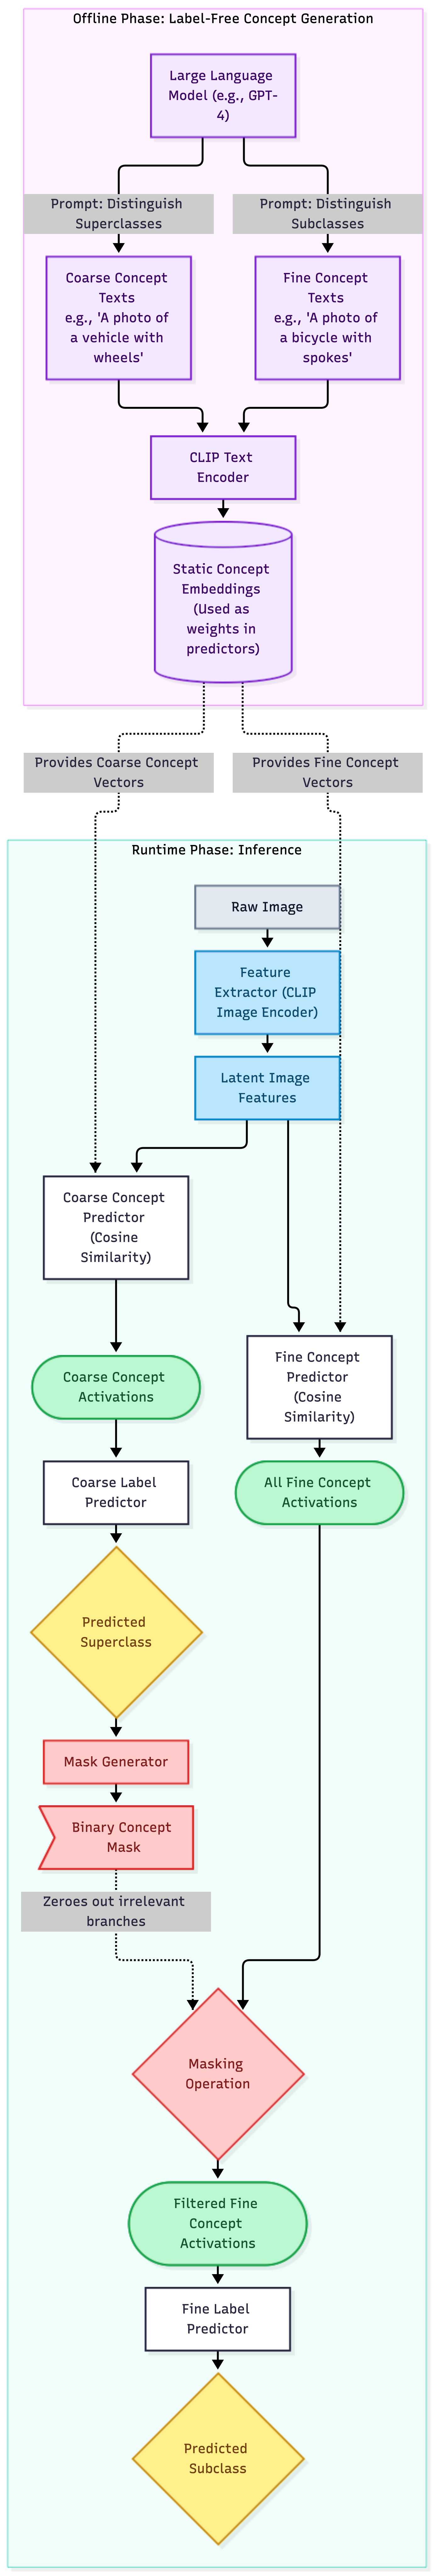
\includegraphics[width=\linewidth, height=\textheight, keepaspectratio]{figures/architecture_ver2.png}
    \caption{Overview of the Hierarchical Coarse-to-Fine Hard Gating Architecture. \\ \small The framework explicitly separates coarse and fine concepts. A superclass prediction acts as a hard mask, dynamically pruning logically incompatible fine-grained concepts before final classification.}
    \label{fig:arch}
\end{figure}

Our architecture (Figure~\ref{fig:arch}) introduces a \textbf{Coarse-to-Fine Hard Gating} mechanism designed to address the aforementioned gaps by strictly imposing a \textbf{dual hierarchy}: a hierarchy at the \textit{class level} (20 superclasses and 100 fine subclasses) and an aligned hierarchy at the \textit{concept level} (coarse concepts and fine concepts). We explicitly constructed a custom High-Resolution CIFAR-100 dataset to retain this rigorous two-tier taxonomy without suffering the degradation of upsampling native 32x32 images, which is necessary to extract high-quality CLIP embeddings.

The methodology unfolds in three phases:
1. \textbf{Label-Free Concept Generation (Concept Hierarchy):} Following the LF-CBM paradigm~\cite{Pastor_2026_tutorial}, we used an LLM to generate two completely separated dictionaries. The \textit{Coarse Concepts} describe broad visual properties suitable for macro-categories, while the \textit{Fine Concepts} capture detailed, class-specific traits.
2. \textbf{Coarse Bottleneck (Class Hierarchy - Level 1):} A coarse logistic regression evaluates the image using \textit{only} the Coarse Concepts to predict one of the 20 superclasses. By completely isolating the coarse bottleneck from fine-grained features, we force the model to reason purely on macro-semantics.
3. \textbf{Hard Gating \& Fine Prediction (Class Hierarchy - Level 2):} The predicted superclass acts as a hard, deterministic mask bridging the two hierarchies. It dynamically sets the activations of all logically incompatible Fine Concepts to zero (e.g., if "Vehicle" is predicted, "fur" or "scales" are nullified). The final fine-grained classification relies exclusively on the "surviving" concepts, guaranteeing logical coherence by design.

\section{Experiments and analysis}
To validate our approach, we first analyze the quality of the generated concepts and then benchmark our Hierarchical CBM (Hier. CBM) against a standard Flat LF-CBM and a black-box CLIP Linear Probe. 

\subsection{Validation of Generated Concepts}
Since our approach relies entirely on Label-Free concept generation, it is crucial that the LLM produces semantically cohesive and distinct concepts. Figure~\ref{fig:per_sc} shows a t-SNE projection of the CLIP text embeddings for the generated coarse concepts. The distinct clustering confirms that CLIP's latent space natively understands the taxonomical separation of the 20 superclasses, independent of our trained model.

\begin{figure}[htbp]
    \centering
    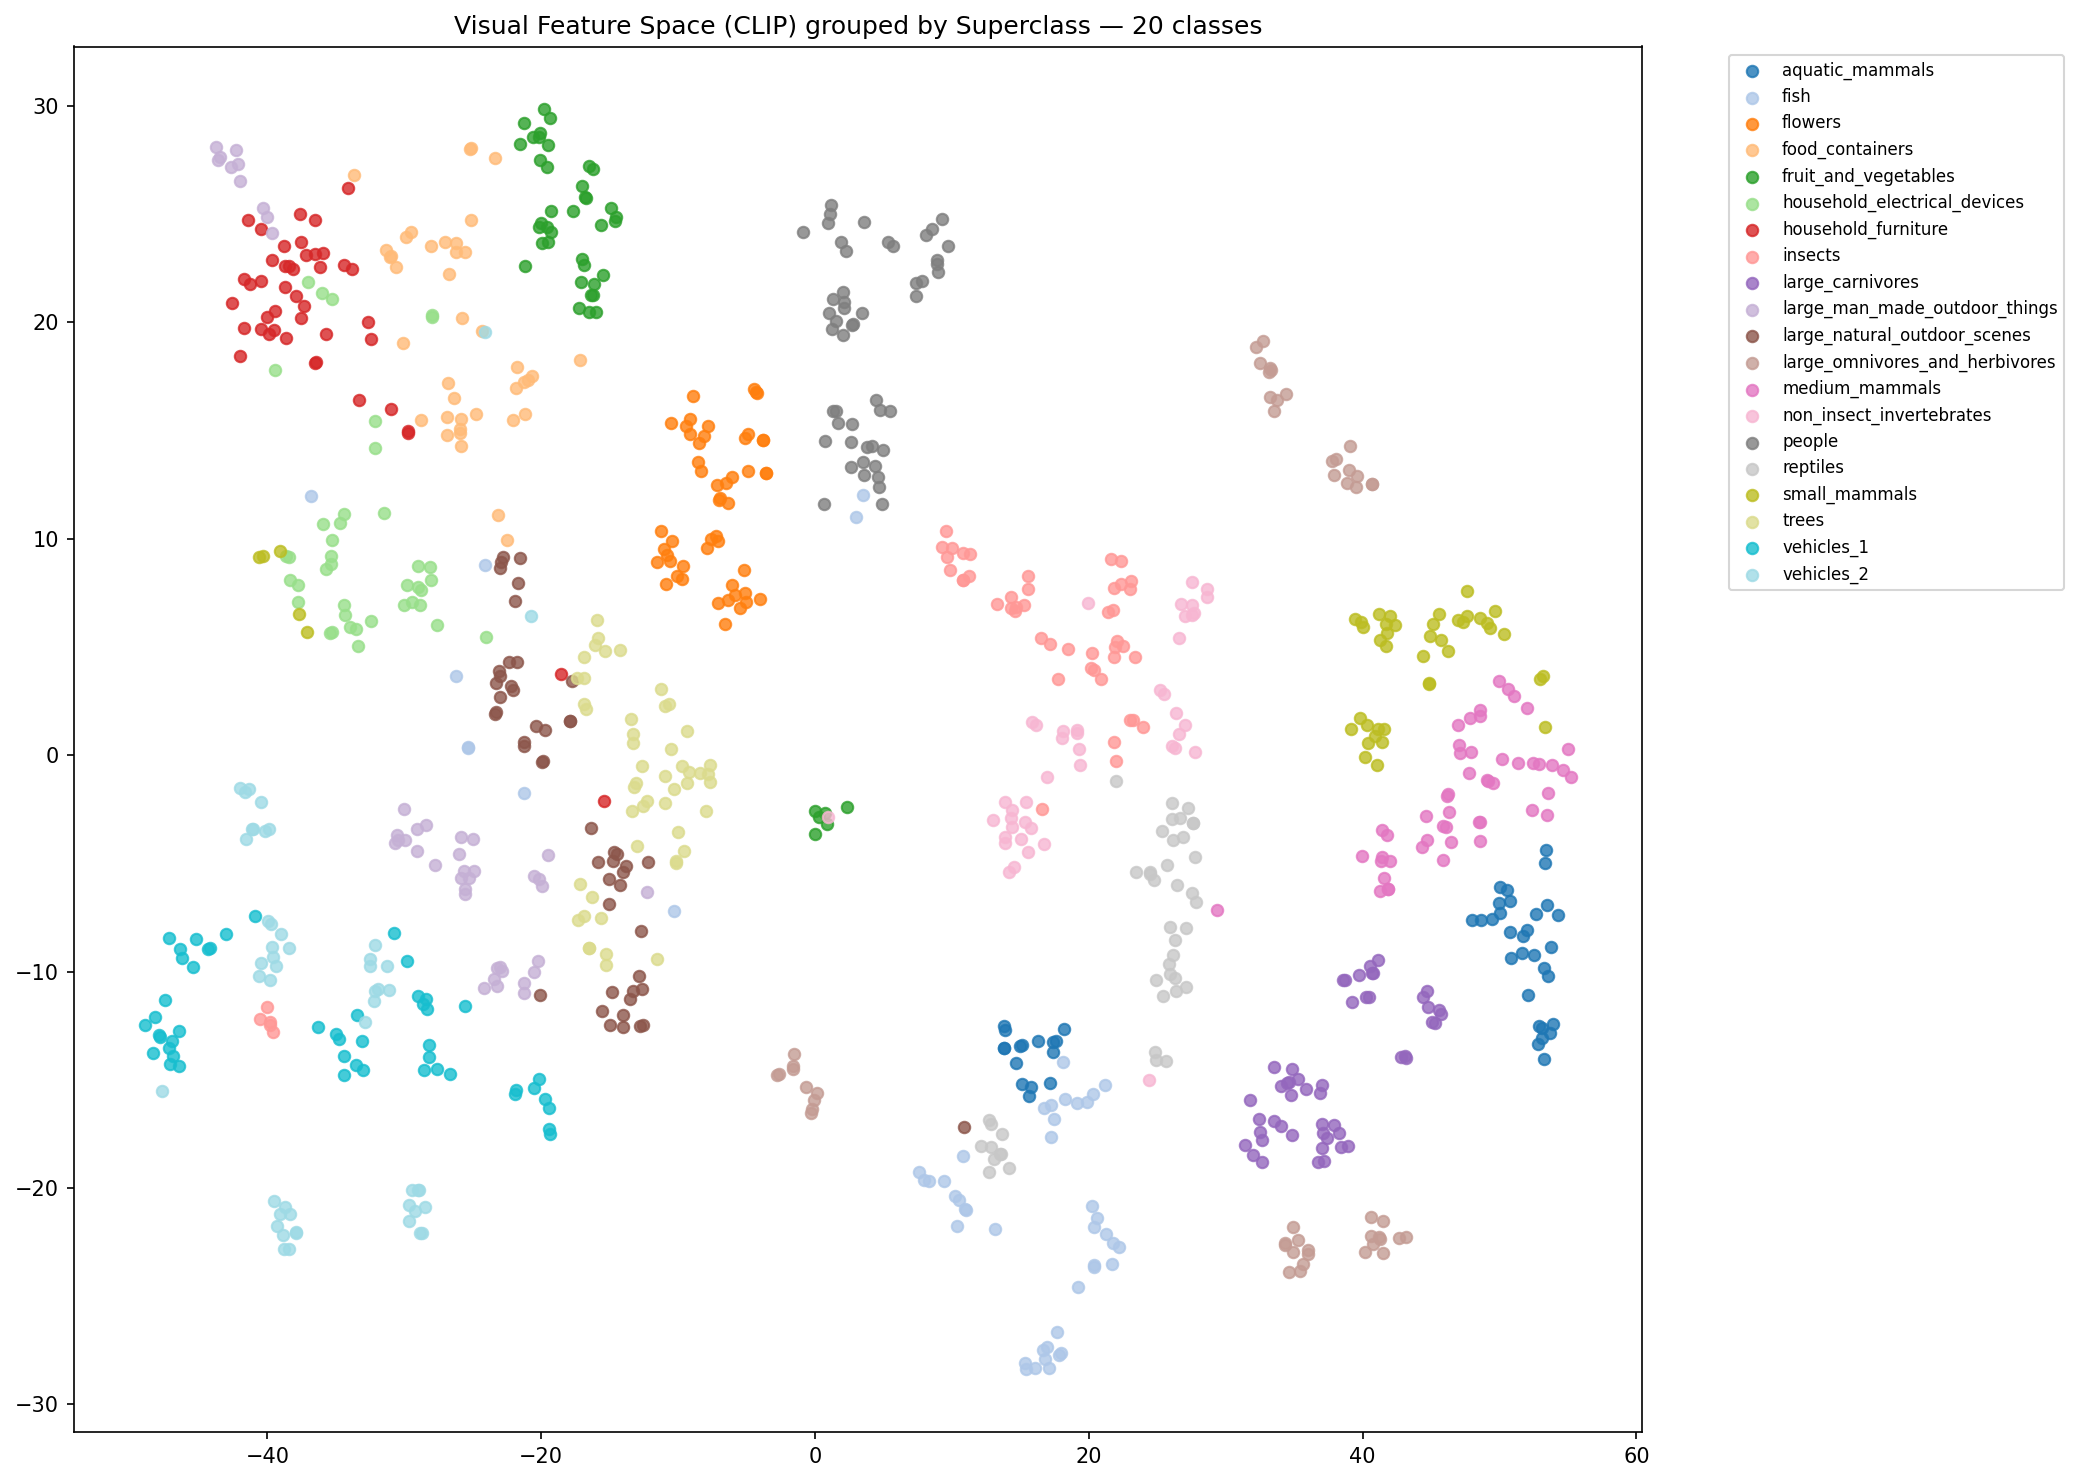
\includegraphics[width=\linewidth]{figures/fig_visual_tsne.png}
    \caption{t-SNE Visualization of the LLM-generated concepts. \\ \small The distinct clusters represent the CLIP text embeddings of the concepts, validating that the LLM successfully generated semantically separable vocabularies for each superclass.}
    \label{fig:per_sc}
\end{figure}

Furthermore, to validate that these textual concepts align with visual inputs, Figure~\ref{fig:oracle} displays the raw cosine similarity (activations) between images from the 'Vehicles 1' superclass and the concept bank. The heatmap demonstrates strong, localized activations for vehicle-related concepts while remaining mostly inactive for irrelevant concepts, validating the quality of the generated text-image alignments prior to training.

\begin{figure}[htbp]
    \centering
    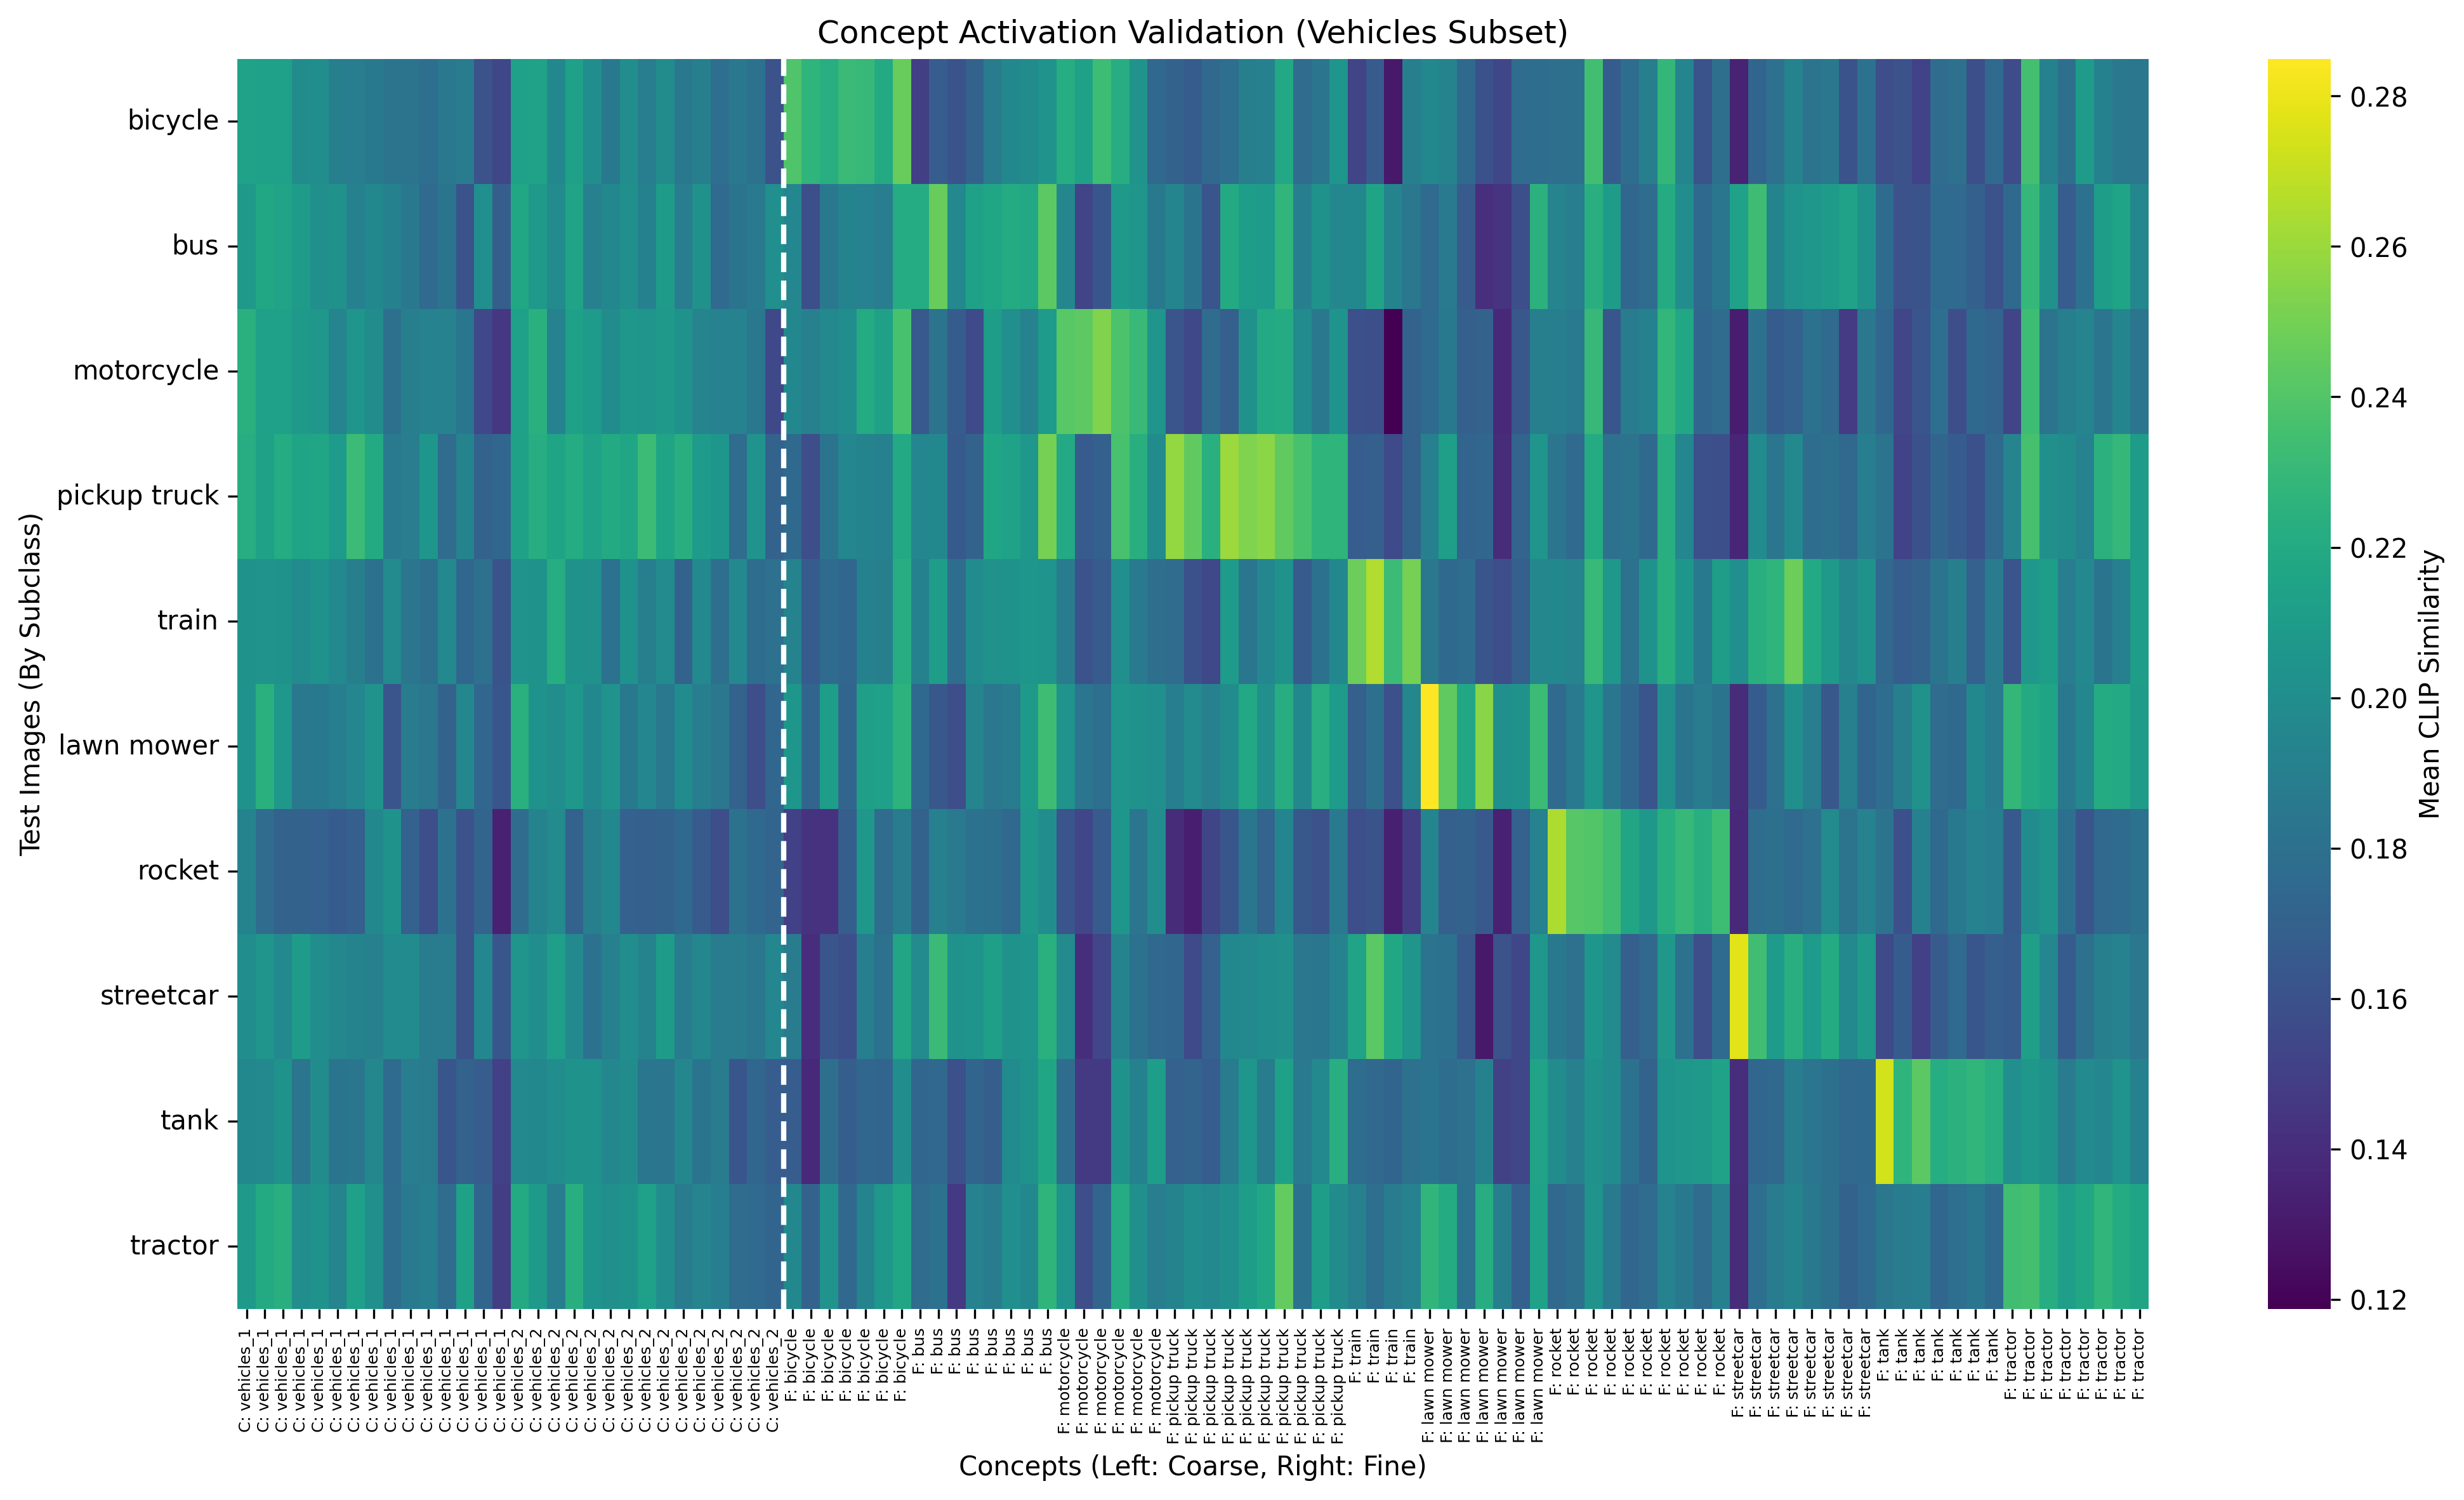
\includegraphics[width=\linewidth]{figures/fig_activation_heatmap_vehicles.png}
    \caption{Concept Activation Heatmap (CLIP Cosine Similarity) for Vehicles. \\ \small This validates the generated concepts by showing that raw images of vehicles strongly activate the correct subset of concepts in CLIP's multimodal space without any fine-tuning.}
    \label{fig:oracle}
\end{figure}

\subsection{Hierarchy-Aware Mistake Evaluation}
Standard Top-1 Accuracy fails to capture the semantic severity of errors. We utilized the Lowest Common Ancestor (LCA) Error Distance, where an error within the same superclass (sibling mistake) has $LCA=1$, and an error across different superclasses (catastrophic mistake) has $LCA=2$.

\begin{figure}[htbp]
    \centering
    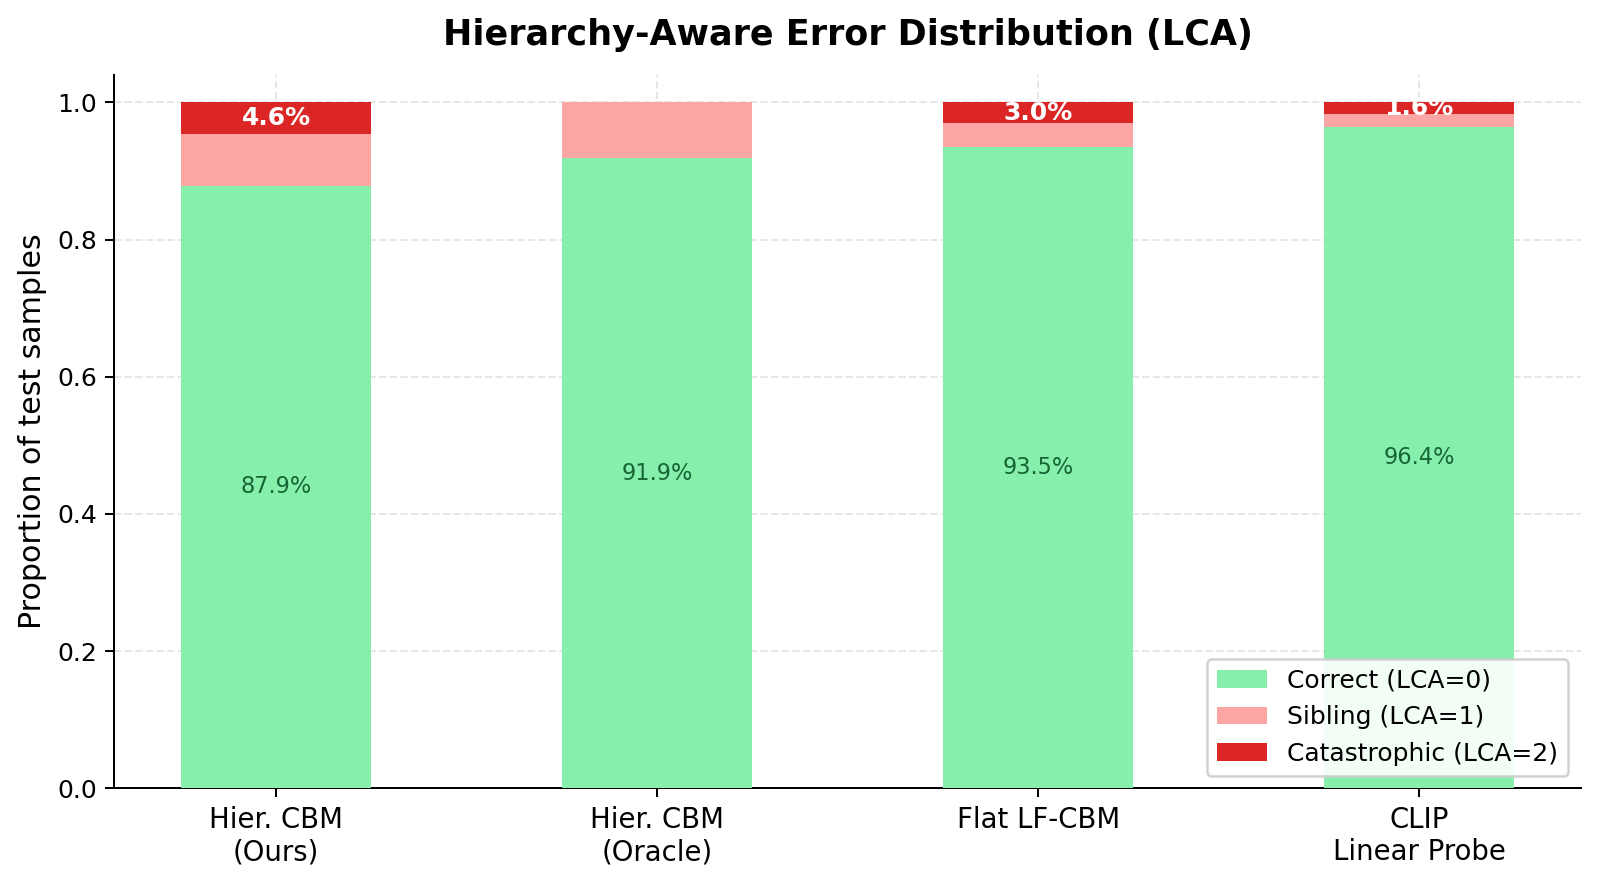
\includegraphics[width=\linewidth]{figures/fig_lca_distribution.png}
    \caption{Hierarchy-Aware Error Distribution (LCA). \\ \small Comparison of error types across models. The Hierarchical CBM (Ours) favors sibling mistakes over catastrophic errors compared to flat baselines.}
    \label{fig:lca}
\end{figure}

As shown in Figure~\ref{fig:lca}, while the Flat LF-CBM has a 3.0\% catastrophic error rate (nearly equal to its sibling mistake rate), our model reduces this to ensure that when it does fail, it fails gracefully within the correct semantic domain.

\subsection{Interpretability and Intervenability}
A fundamental promise of CBMs is the ability for humans to intervene and correct the model's intermediate reasoning. We simulated an \textit{Oracle Intervention}, representing a domain expert correcting the coarse superclass prediction. 

\begin{table}[htbp]
\caption{Performance Comparison across Models. \\ \small Results highlight the Oracle's perfect mitigation of catastrophic errors and its minimal active concept footprint.}
\label{tab:results}
\resizebox{\linewidth}{!}{%
\begin{tabular}{lrrrr}
\toprule
\textbf{Metric} & \textbf{Hier. CBM (Ours)} & \textbf{Hier. CBM (Oracle)} & \textbf{Flat LF-CBM} & \textbf{CLIP Linear Probe} \\
\midrule
Top-1 Acc. & 0.8786 & \textbf{0.9191} & 0.9350 & \textbf{0.9642} \\
Top-3 Acc. & 0.9489 & N/A & 0.9915 & \textbf{0.9949} \\
Avg Active Conc. & (46.0+5.4)/2 & \textbf{5.4} & 10.2 & 512 (dim) \\
Avg LCA Dist. & 0.1672 & 0.0809 & 0.0948 & \textbf{0.0521} \\
\% Sibling (LCA=1) & 0.076 & 0.081 & 0.035 & 0.019 \\
\% Catastrophic (LCA=2) & 0.046 & 0.000 & 0.030 & 0.016 \\
\bottomrule
\end{tabular}}
\end{table}

Table~\ref{tab:results} reveals the profound impact of our hard-gating architecture under intervention. The key takeaway is that a single high-level Oracle correction on the superclass cascades down through the hard gate, boosting the model's overall accuracy to 91.91\%. This allows our interpretable Hierarchical CBM to close the performance gap and achieve an accuracy that is highly competitive with the black-box CLIP probe (96.42\%) and the standard Flat LF-CBM (93.50\%), while maintaining a strict semantic taxonomy that naturally precludes any cross-superclass ($LCA=2$) errors.

More importantly, the hard gate drastically reduces the cognitive load required to understand the model's final decision. While the model initially uses an average of 46 concepts to find the superclass, once the superclass is fixed (either by the network or the Oracle), it requires an average of only \textbf{5.4 active fine concepts} to determine the final class. Figure~\ref{fig:sparsity} illustrates this sparsity vs accuracy trade-off, placing our Oracle intervention firmly in the high interpretability zone.

\begin{figure}[htbp]
    \centering
    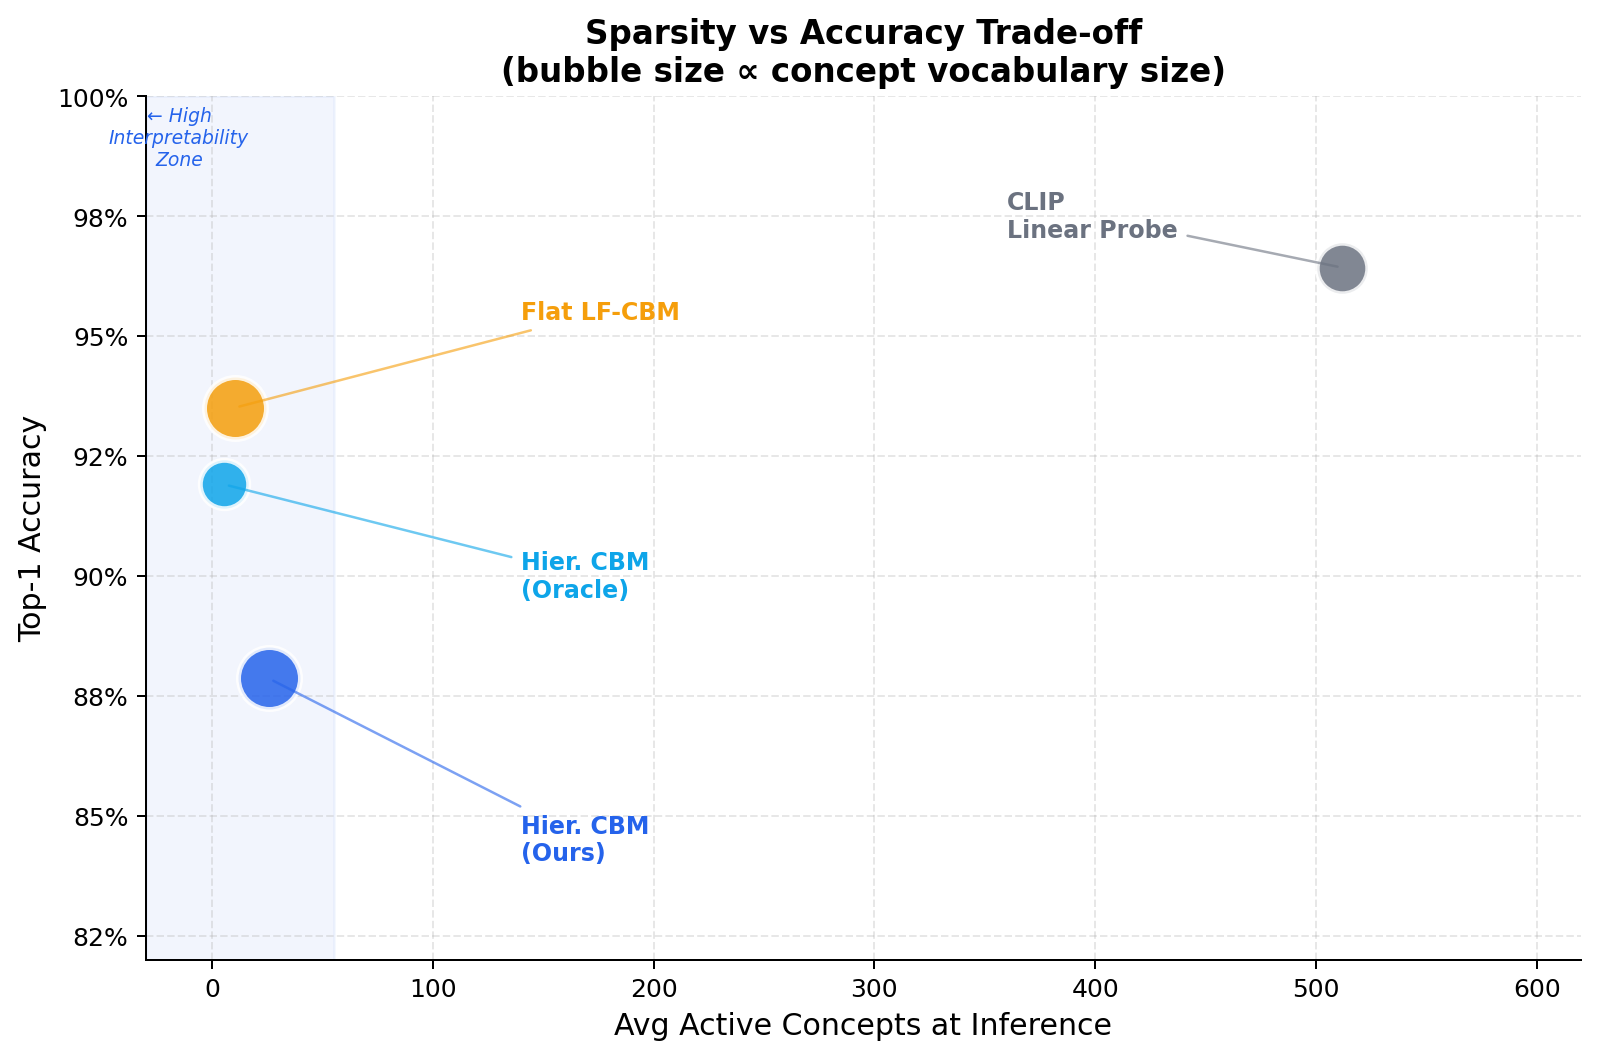
\includegraphics[width=\linewidth]{figures/fig_sparsity_bubble.png}
    \caption{Sparsity vs Accuracy Bubble Chart. \\ \small The bubble size represents the average active concept vocabulary. The Oracle intervention achieves high accuracy while requiring an extremely sparse set of concepts (5.4 on average).}
    \label{fig:sparsity}
\end{figure}

\begin{figure}[htbp]
    \centering
    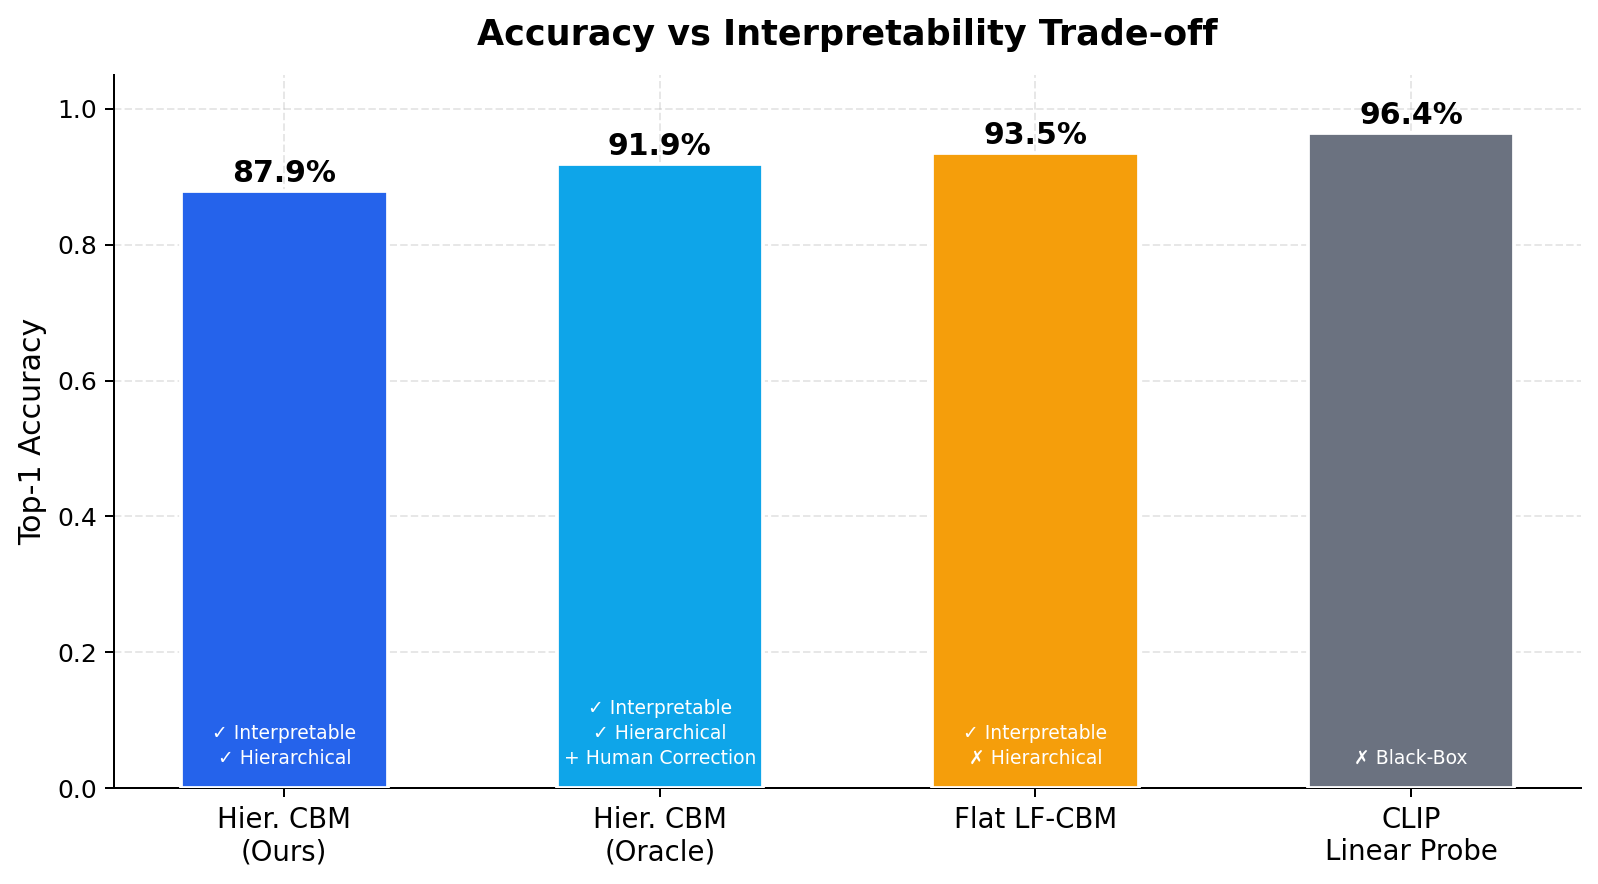
\includegraphics[width=\linewidth]{figures/fig_accuracy_tradeoff.png}
    \caption{Accuracy vs Interpretability Trade-off. \\ \small Visualizing the cost of transparency. While the Hierarchical CBM sacrifices some absolute accuracy compared to the CLIP probe, it gains perfect logical transparency and intervenability.}
    \label{fig:tradeoff}
\end{figure}

Figure~\ref{fig:tradeoff} highlights the overarching trade-off of our system. Full interpretability and adherence to a strict hierarchy cost approximately 8.5\% in top-1 accuracy compared to a black-box CLIP probe, but in exchange, the model guarantees logical transparency, eliminates concept bleeding, and provides a highly effective vector for human intervention.

\section{Conclusions}
In this project, we proposed a Hierarchical Coarse-to-Fine Label-Free Concept Bottleneck Model to address the limitations of flat CBM representations and evaluation strategies. By embedding a rigorous dual-level hierarchy spanning both class labels and conceptual features, and introducing a dynamic hard-gating mechanism, we effectively bridged the gap between structural concept definitions and model inference. Our evaluation using hierarchy-aware LCA metrics demonstrates that our architecture fails more gracefully than flat alternatives and is highly receptive to human intervention, reducing cognitive load to just over 5 active concepts per decision.

\bibliographystyle{ACM-Reference-Format}
\bibliography{biblio}

\end{document}
